
\chapter{Elemente der Stochastik}

\section{Grundbegriffe}

\subsection{Ereignisse}

Die Wahrscheinlichkeitstheorie beschäftigt sich mit
\emph{Zufallsexperimenten}. Darunter versteht man ein Experiment
mit zufälligem Ausgang, das, um der Wissenschaftlichkeit genüge zu tun,
unter genau definierten Versuchsbedingungen durchgeführt wird.
Der Ausgang führt immer zu einem \emph{Ergebnis}. Alle erreichbaren
Ergebnisse fasst man zur \emph{Ergebnismenge} zusammen. Allgemeiner
genügt es, wenn jedes Ergebnis in der Ergebnismenge liegt, wobei diese
aber auch Elemente enthalten darf, die das Experiment niemals abwirft.
Jede Teilmenge der Ergebnismenge nennt man ein \emph{Ereignis}\index{Ereignis}.
Die Potenzmenge der Ergebnismenge heißt \emph{Ereignisraum}, sie
besteht aus allen denkbaren Ereignissen. Man sagt, ein Ereignis sei
eingetreten, wenn das Ergebnis des Versuchs im diesem Ereignis liegt.

Zu beachten ist, dass wir dabei eine endliche oder höchstens
abzählbar unendliche Ergebnismenge voraussetzen. Bei überabzählbaren
Ergebnismengen kommt es zu Unwägbarkeiten, deren Klärung Gegenstand der
Maßtheorie ist.

Ein schlichtes Experiment bietet der Wurf des Spielwürfels, eines mit
Augenzahlen beschrifteten regelmäßigen Hexaeders. Die Ergebnismenge
wird als
\[\Omega := \{1, 2, 3, 4, 5, 6\}\]
festgelegt. Betrachten wir die drei Ereignisse
\[A := \{2\},\quad B := \{1,2\},\quad C:=\{1,3\}.\]
Ist $\omega=2$ das Ergebnis des Versuchs, sind die Ereignisse $A,B$
eingetreten. Zwei Ereignisse, die niemals gleichzeitig eintreten,
heißen \emph{disjunkt}. So sind die $A,C$ disjunkt, weil ihre
Schnittmenge leer ist.

\subsection{Nochmals Indikatorfunktionen}

In diesem Abschnitt will ich nochmals näher auf Indikatorfunktionen%
\index{Indikatorfunktion} eingehen. Sie bieten in der Kombinatorik und
in der Wahrscheinlichkeitsrechnung beim Rechnen mit Summen ein Hilfsmittel,
das bestimmte Umformungen leichter verständlich macht.

\begin{table}
\centering
\caption{Regeln für die Iverson-Klammerung}
\label{tab:Iverson}
\begin{tabular}{r@{\;}l@{\qquad}r@{\;}l}
\toprule
$[\bot]$ & $= 0$ & $[a\land b]$ & $= [a]\cdot [b]$\\
$[\top]$ & $= 1$ & $[a\lor b]$ & $= [a] + [b] - [a]\cdot [b]$\\
$[\lnot a]$ & $= 1 - [a]$ & $[a\oplus b]$ & $= |[a] - [b]|$\\
\bottomrule
\end{tabular}
\end{table}

Wir rekapitulieren nochmals die Iverson"=Klammerung, die Wahrheitswerte
in die Menge der Zahlen einbettet. Für jede Aussage $E$ ist
\[[A] := \begin{cases}
0, & \text{wenn $A$ falsch ist,}\\
1, & \text{wenn $A$ wahr ist.}
\end{cases}\]
Hiermit wird zu jeder Menge $M\subseteq\Omega$ die Indikatorfunktion als
\[1_M\colon\Omega\to\{0,1\},\quad 1_M(\omega) := [\omega\in M]\]
festgelegt. Für die Iverson"=Klammerung gelten die Regeln in Tabelle
\ref{tab:Iverson}, die man leicht per Wahrheitstafel nachrechnen kann.
Es wäre zu bemerken, dass man damit genau die Einbettung der
Aussagenlogik in die gewöhnliche Algebra erhält, wie Boole sie
darstellte.
\begin{Satz}\label{Indikatorf-Vereinigung2}
Für jedes $\omega$ gilt
\[1_{A\cup B}(\omega) = 1_A(\omega) + 1_B(\omega) - 1_{A\cap B}(\omega).\]
\end{Satz}
\begin{Beweis}
Laut Definition ist die Gleichung äquivalent zur Gleichung
\begin{align*}
&[\omega\in A\cup B] = [\omega\in A] + [\omega\in B] - [\omega\in A\cap B]\\
\iff & [\omega\in A\lor\omega\in B] = [\omega\in A] + [\omega\in B] - [\omega\in A\land\omega\in B].
\end{align*}
Diese gilt aber gerade laut Tabelle \ref{tab:Iverson}.\,\qedsymbol
\end{Beweis}

\noindent
Die Indikatorfunktion einer endlichen Mengen ermöglicht es, die
Anzahl ihrer Elemente als eine Summe darzustellen. Man sieht sofort ein,
dass $|A| = \sum_{\omega\in\Omega} 1_A(\omega)$ für eine Menge $A\subseteq\Omega$
gelten muss, was recht trivial erscheinen mag. Infolge erhält man aber aus
Satz \ref{Indikatorf-Vereinigung2} unverzüglich den Korollar
\[|A\cup B| = |A|+|B|-|A\cap B|.\]

\subsection{Wahrscheinlichkeiten}

Man kann nicht voraussagen, wie ein Experiment ausgehen wird. Das
Wahrscheinlichkeitsmaß liefert dennoch ein Maß dafür, wie sicher der
Eintritt eines Ereignisses ist. Wahrscheinlichkeit wird tiefergründig
verständlich, wenn dasselbe Zufallsexperiment abermals wiederholt wird.
Wir zählen, wie häufig ein Elementarereignis eingetreten ist.

Es sei ein Versuch $n$ mal durchgeführt worden, was zu den Ergebnissen
$a_i$ für $i=1$ bis $i=n$ geführt hat. Wir definieren die \emph{relative
Häufigkeit}\index{relative Haeufigkeit@relative Häufigkeit}
des Ereignisses $A$ als die Zahl
\[r_{n,a}(A) := \frac{1}{n}|\{i\in\{1,\ldots,n\}\mid a_i\in A\}|.\]
Relative Häufigkeiten bieten bei hinreichend großem $n$ eine Näherung
für die Wahrscheinlichkeit. Zur Vermessung eines Würfels wird man
diesen also möglichst oft werfen wollen. Man erhält so die relativen
Häufigkeiten der Elementarereignisse, und damit näherungsweise auch
ihre Wahrscheinlichkeiten. So lässt sich feststellen, ob ein
Würfel gezinkt wurde.

Fassen wir $a$ als Funktion $i\mapsto a_i$ auf, können wir schreiben
\[\{i\mid a_i\in A\} = \{i\mid i\in a^{-1}(A)\} = a^{-1}(A).\]
Für disjunkte Ereignisse $A,B$ erhält man nun
\begin{align*}
r_{n,a}(A\cup B) &= \tfrac{1}{n}|a^{-1}(A\cup B)|
= \tfrac{1}{n}|a^{-1}(A)\cup a^{-1}(B)|\\
&= \tfrac{1}{n}|a^{-1}(A)| + \tfrac{1}{n}|a^{-1}(B)|
= r_{n,a}(A) + r_{n,a}(B).
\end{align*}
Weil $\Omega$ die Zielmenge von $a$ ist, muss $a_i\in\Omega$
für jedes $i\in\Omega$ gelten, also $|a^{-1}(\Omega)|=n$. Somit gilt
\[r_{n,a}(\Omega) = 1,\]
unabhängig davon, wie groß die Zahl $n$ ist. Und weil sich aus der
Definition von $a$ unmittelbar $0\le |a^{-1}(A)|\le n$ ergibt, besteht der
Sachverhalt
\[0\le r_{n,a}(A)\le 1.\]
Weiterhin ergibt sich, dass sich die Häufigkeit monoton bezüglich der
Inklusion verhält, das heißt, es besteht die Implikation
\[A\subseteq B\Rightarrow r_{n,a}(A)\le r_{n,b}(B).\]
Laut Satz \ref{Monotonie-Bild-Urbild} folgt nämlich $a^{-1}(A)\subseteq a^{-1}(B)$
aus $A\subseteq B$. Daraufhin ergibt sich $|a^{-1}(A)|\le |a^{-1}(B)|$.

Die Vorstellung von der Wahrscheinlichkeit\index{Wahrscheinlichkeit}
besteht darin, dass sich die relative Häufigkeit ihr mit steigender
Anzahl der Versuche immer weiter nähert. Dies bedeutet, es wird meistens
$P(A)\approx r_{n,a}(A)$ für hinreichend großes $n$ gelten. Die bisher
erläuterten Eigenschaften von $r_{r,a}$ sollten diesbezüglich für $P$
bestehen bleiben, da diese nicht von $n$ abhängen.

Untermauert wird diese Überlegung durch das \emph{Gesetz der großen
Zahlen}. Es zu diskutieren, würde an dieser Stelle aber zu weit führen.
Zum einem müsste dafür zunächst der Begriff des Grenzwertes eingeführt
werden. Zum anderen ist der Grenzwertbegriff der Analysis nicht in direkter
Weise auf den Sachverhalt anwendbar. Auf dessen Basis müssten zunächst
die Konvergenzbegriffe für Zufallsgrößen erörtert werden.

Stattdessen wird der Begriff des Wahrscheinlichkeitsmaßes erst einmal
axiomatisch eingeführt. Darauf aufbauend, was unter einer Zufallsgröße
zu verstehen sei.

\begin{Definition}[Endlicher Wahrscheinlichkeitsraum]\newlinefirst
Sei $\Omega$ eine nichtleere endliche Menge. Das Paar $(\Omega,P)$ nennt
man einen \emph{endlichen Wahrscheinlichkeitsraum}, wenn
\[P\colon\powerset(\Omega)\to\R,\quad P(A) := \sum_{\omega\in A}P(\{\omega\})\]
die Eigenschaften $\mathrm{Bild}(P)\subseteq [0,1]$ und $P(\Omega)=1$ besitzt.
\end{Definition}

\noindent
Ein endlicher Wahrscheinlichkeitsraum kann alternativ auch durch die
kolmogorowschen Axiome charakterisiert werden. Der Vorteil besteht darin,
dass diese später auch unter allgemeineren Umständen gültig bleiben.

\begin{Satz}[Axiome von Kolmogorow]\label{Axiome-Kolmogorow}%
\index{Axiome von Kolmogorow}\index{Kolmogorow, Axiome von}\newlinefirst
Sei $\Omega$ eine nichtleere endliche Menge und
$P\colon\powerset(\Omega)\to\R$. Es ist $(\Omega,P)$ genau dann
ein endlicher Wahrscheinlichkeitsraum, wenn
\begin{align*}
& P(A) \ge 0\;\text{für}\;A\subseteq\Omega,\\
& P(\Omega) = 1,\\
& P(A\cup B) = P(A) + P(B)\;\text{für}\;A,B\subseteq\Omega\;
\text{mit}\;A\cap B=\emptyset.
\end{align*}
\end{Satz}
\begin{Beweis}
Es sei $(\Omega,P)$ ein endlicher Wahrscheinlichkeitsraum.
Mit $A\cap B=\emptyset$ gilt für die Indikatorfunktionen
gemäß Satz \ref{Indikatorf-Vereinigung2} die Gleichung
\[1_{A\cup B}(\omega) = 1_A(\omega) + 1_B(\omega).\]
Somit gelingt die Rechnung
\begin{gather*}
P(A\cup B) = \sum_{\omega\in A\cup B}P(\{\omega\})
= \sum_{\omega\in\Omega}P(\{\omega\})1_{A\cup B}(\omega)\\
= \sum_{\omega\in\Omega}P(\{\omega\})(1_A(\omega)+1_B(\omega))
= \sum_{\omega\in\Omega}P(\{\omega\})1_A(\omega)+
\sum_{\omega\in\Omega}P(\{\omega\})1_B(\omega)\\
= \sum_{\omega\in A}P(\{\omega\}) + \sum_{\omega\in B}P(\{\omega\})
= P(A) + P(B).
\end{gather*}
Umgekehrt erfülle $(\Omega,P)$ die kolmogorowschen Axiome. Da die
elementaren Ereignisse $\{\omega\}$ paarweise disjunkt sind, ergibt sich
\[P(A) = P(\bigcup_{\omega\in A}\{\omega\})
= \sum_{\omega\in A} P(\{\omega\}).\]
Mit dieser Summenformel erhält man die Aussage $P(A)\le 1$ nun als Korollar
aus Satz \ref{Monotonie-P} mit $A:=A$ und $B:=\Omega$.\,\qedsymbol
\end{Beweis}

\begin{Satz}\label{Monotonie-P}
Gilt $A\subseteq B$, so ist $P(A)\le P(B)$.
\end{Satz}
\begin{Beweis}
Mit $A\subseteq B$ ist $1_A(\omega)\le 1_B(\omega)$ für jedes $\omega\in\Omega$.
Ergo gilt
\[P(A) = \sum_{\omega\in\Omega} P(\{\omega\})1_A(\omega)
\le \sum_{\omega\in\Omega} P(\{\omega\})1_B(\omega) = P(B).\,\qedsymbol\]
\end{Beweis}

\noindent
Die Vorstellung von der Wahrscheinlichkeit als Chance oder Risiko
mag aufgrund ihres Charakters als Unwägbarkeit schwierig fassbar sein.
Der frequentistische Wahrscheinlichkeitsbegriff wird hingegen mit seiner
Erklärung von Wahrscheinlichkeit als relative Häufigkeit bei großer
Zahl der Versuche schon greifbarer. Mir fällt dazu eine Sichtweise ein,
die sich dem zufälligen Charakter so weit entzieht wie es nur geht.
Lässt man die große Zahl der Versuche parallel ablaufen, gibt die
die Wahrscheinlichkeit den \emph{Anteil} der Ergebnisse an, die in
der jeweiligen Teilmenge enthalten sind. Werdem zum Beispiel eine
Million Spielwürfel auf einmal geworfen, wird jede der Augenzahlen
voraussichtlich näherungsweise mit dem Anteil $\frac{1}{6}$ vorkommen.
Oder denkt man sich eine Population von unzählig vielen Individuen,
und erhält jedes die gleiche Wahrscheinlichkeit $P(A)$, ein
bestimmtes Merkmal $A$ zu besitzen, wird man in der Population einen
Anteil von näherungsweise $P(A)$ Individuen mit dem Merkmal $A$ vorfinden.

Das Wahrscheinlichkeitsmaß $P$ erfüllt einige Gesetzmäßigkeiten, die
elementar aus den Axiomen ableitbar sind.

\begin{Satz}
Allgemein gilt $P(A^\compc) = 1 - P(A)$.
\end{Satz}
\begin{Beweis}
Da $\Omega = A\cup A^\compc$ eine Zerlegung von $\Omega$ in zwei
disjunkte Mengen ist, erhält man $P(\Omega)=P(A)+P(A^\compc)$.
Die Gleichung $P(\Omega)=1$ wird daraufhin kurzum nach $P(A^\compc)$
umgeformt.\,\qedsymbol
\end{Beweis}

\begin{Satz}\label{Inklusion-Exklusion-zwei}
Allgemein gilt $P(A\cup B) = P(A) + P(B) - P(A\cap B)$.
\end{Satz}
\begin{Beweis}
Vermittels Satz \ref{Indikatorf-Vereinigung2} formt man wie im Beweis
von Satz \ref{Axiome-Kolmogorow} die Summenformel für
$P(A\cup B)$ um.\,\qedsymbol
\end{Beweis}

\noindent
Alternativ kann die Identität folgendermaßen direkt aus dem dritten
kolmogorowschen Axiom abgeleitet werden, ohne den Weg über die Summenformel
zu gehen. Man überzeugt sich mühelos davon, dass $A$ via%
\[A = A\cap\Omega = A\cap(B\cup B^\compc) = (A\cap B)\cup (A\cap B^\compc)\]
als Vereinigung disjunkter Mengen dargestellt werden kann. Ergo gilt%
\[P(A) = P(A\cap B) + P(A\cap B^\compc).\]
Analog bekommt man
\[A\cup B = (A\cup B)\cap (B\cup B^\compc) =
((A\cup B)\cap B)\cup ((A\cup B)\cap B^\compc)\]
als Vereinigung disjunkter Mengen. Der letzte Term vereinfacht sich
mit dem Absorptionsgesetz $(A\cup B)\cap B = B$ und $(A\cup B)\cap B^\compc
= A\cap B^\compc$ via Distributivgesetz, Komplementärgesetz und
Neutralitätsgesetz. Demzufolge gilt%
\[P(A\cup B) = P(B) + P(A\cap B^\compc).\]
Löst man die vorherige Gleichung nun nach $P(A\cap B^\compc)$ auf
und setzt sie in diese ein, findet sich schließlich Satz
\ref{Inklusion-Exklusion-zwei}.

Vermittels Satz \ref{Inklusion-Exklusion-zwei} wird unschwer die Formel
\[P(A\cup B\cup C) = P(A) + P(B) + P(C)
- P(A\cap B) - P(A\cap C) - P(B\cap C) + P(A\cap B\cap C)\]
gewonnen. Umgekehrt kann Satz \ref{Inklusion-Exklusion-zwei} unmittelbar
aus ihr zurückgewonnen werden, indem einfach $C:=\emptyset$ gesetzt
wird. Diese Formeln folgen einem allgemeinen Prinzip, das
allgemein für Vereinigungen endlich vieler Mengen gilt, -- man spricht
von der \emph{Siebformel}, auch als \emph{Prinzip der Inklusion und Exklusion}
geläufig.

Zur gründlicheren Erfassung des Prinzips will ich einen Beweis
der Siebformel aufzeigen, der allerdings ein wenig kompliziert ausfällt.
Zunächst benötigen wir einen Hilfssatz für die Handhabung der
Indikatorfunktionen.

\begin{Satz}\label{prod-1-plus}
Es gilt $\prod_{i=1}^n (1+a_i) = \sum_{J\subseteq\{1,\ldots,n\}}\prod_{j\in J} a_j$.
\end{Satz}
\begin{Beweis}
Induktion über $n$. Im Anfang $n=0$ gilt $\{1,\ldots,n\}=\emptyset$,
womit $J=\emptyset$ die einzige Teilmenge ist. Auf beiden Seiten steht
also das leere Produkt, dessen Wert eins ist.

Zum Schritt rechnet man
\begin{align*}
\prod_{i=1}^{n+1} (1+a_i) &= (1+a_{n+1})\prod_{i=1}^n (1+a_i)
\stackrel{\mathrm{IV}}= (1+a_{n+1})\sum_{J\subseteq\{1,\ldots,n\}}\prod_{j\in J} a_j\\
&= \sum_{J\subseteq\{1,\ldots,n\}}\prod_{j\in J} a_j
+ \sum_{J\subseteq\{1,\ldots,n\}}\prod_{j\in J\cup\{n+1\}} a_j
= \sum_{J\subseteq\{1,\ldots,n+1\}}\prod_{j\in J} a_j.
\end{align*}
Die letzte Umformung ergibt sich daraus, dass laut Satz
\ref{Potenzmenge-rekursiv} gilt
\[J\subseteq\{1,\ldots,n+1\} \,\Leftrightarrow\,\,
J\in\mathcal P(\{1,\ldots,n\})\uplus\{A\cup\{n+1\}\mid A\subseteq\{1,\ldots,n\}\}.\,\qedsymbol\]
\end{Beweis}

\begin{Satz}\label{prod-1-minus}
Es gilt $\prod_{i=1}^n (1-a_i) = \sum_{J\subseteq\{1,\ldots,n\}}(-1)^{|J|}\prod_{j\in J} a_j$.
\end{Satz}
\begin{Beweis}
Ergibt sich als Korollar aus Satz \ref{prod-1-plus}
mit $\prod_{j\in J} (ca_j) = c^{|J|}\prod_{j\in J} a_j$
für jede Konstante $c$, wobei mit $|J|$ die Anzahl der Elemente von $J$ gemeint ist.\,\qedsymbol
\end{Beweis}

\begin{Satz}[Siebformel]\newlinefirst
Es gilt $\displaystyle P(\bigcup_{i=1}^n A_i)
= \sum_{\mathclap{\substack{J\subseteq\{1,\ldots,n\}\\ J\ne\emptyset}}}
(-1)^{|J|+1}P(\bigcap_{j\in J} A_j)$.
\end{Satz}
\begin{Beweis}
Laut Satz \ref{prod-1-minus} gilt
\[\prod_{i=1}^n 1_{\Omega\setminus A_i}(\omega)
= \prod_{i=1}^n (1-1_{A_i}(\omega))
= \sum_{\mathclap{J\subseteq\{1,\ldots,n\}}}(-1)^{|J|}\prod_{j\in J}1_{A_j}(\omega),\]
also
\[1_{\Omega\setminus\bigcup_{i=1}^n A_i}(\omega)
= 1_{\bigcap_{i=1}^n\Omega\setminus A_i}(\omega)
= \sum_{\mathclap{J\subseteq\{1,\ldots,n\}}}(-1)^{|J|}1_{\bigcap_{j\in J} A_j}(\omega).\]
Ergo gilt
\begin{align*}
1 - P(\bigcup_{i=1}^n A_i) &= P(\Omega\setminus\bigcup_{i=1}^n A_i)
= \sum_{\omega\in\Omega}P(\{\omega\})1_{\Omega\setminus\bigcup_{i=1}^n A_i}\\
&= \sum_{\mathclap{J\subseteq\{1,\ldots,n\}}}(-1)^{|J|}\sum_{\omega\in\Omega}
P(\{\omega\})1_{\bigcap_{j\in J} A_j}(\omega)
= \sum_{\mathclap{J\subseteq\{1,\ldots,n\}}}(-1)^{|J|}P(\bigcap_{j\in J} A_j).
\end{align*}
Im Fall $J=\emptyset$ gilt $\bigcap_{j\in J} A_j = \Omega$, deren
Wahrscheinlichkeit eins ist. Man subtrahiert nun eins auf beiden
Seiten, und multipliziert daraufhin beide Seiten mit $-1$.\,\qedsymbol
\end{Beweis}

\newpage
\subsection{Gleichverteilungen}

Viele Zufallsexperimente entstehen aus einer Zusammensetzung vermittels
Gegenständen, die einer Gleichverteilung unterliegen, wo also jedes der
elementaren Ereignisse gleich wahrscheinlich ist. Zum Beispiel ist dies
beim Wurf einer idealen Münze, beim Wurf eines idealen Würfels, bei
der Ziehung einer Karte aus einem gut durchmischten Stapel nummerierter
Karten oder bei der Ziehung einer Kugel aus einer Ansammlung nummerierter
Kugeln der Fall. Auch ein Zufallszahlgenerator mit einer bestimmten Verteilung
lässt sich vermittels bestimmter Algorithmen aus einem gleichverteilten
Generator aufbauen.

Wir nehmen nun für eine Weile die Position ein, dass auf unterster Ebene
immer eine Gleichverteilung herrscht. Wie sich herausstellt, ist diese
These unhaltbar. Das ist aber nicht weiter schlimm, denn auch dieser
eingeschränkte Wahrscheinlichkeitsbegriff zeigt sich bisweilen recht
vielfältig.

\begin{Definition}[Laplace-Experiment]\newlinefirst
Ein \emph{Laplace-Experiment}\index{Laplace-Experiment} ist ein
Zufallsexperiment, bei dem die elementaren Ereignisse alle gleich
wahrscheinlich sind.
\end{Definition}

\noindent
Der Wahrscheinlichkeitsraum $(\Omega,P)$ eines Laplace"=Experiments
hat also die Eigenschaft $P(\{\omega\})=c$ für jedes $\omega\in\Omega$,
wobei $c$ eine Konstante ist.

\begin{Satz}
Herrscht in $(\Omega,P)$ Gleichverteilung, gilt $P(A) = \frac{|A|}{|\Omega|}$.
\end{Satz}
\begin{Beweis}
Man stellt das Ereignis $A$ als Vereinigung der disjunkten elementaren
Ereignisse dar. Diesbezüglich ergibt sich die Umformung
\[P(A) = P(\bigcup_{\omega\in A}\{\omega\})
= \sum_{\omega\in A}P(\{\omega\}) = \sum_{\omega\in A} c
= c\sum_{\omega\in A} 1 = c\cdot |A|.\]
Speziell gilt $1=P(\Omega)=c\cdot |\Omega|$, womit
$c=\frac{1}{|\Omega|}$ sein muss.\,\qedsymbol
\end{Beweis}

\subsection{Zufallsgrößen}

Eine \emph{Zufallsgröße}\index{Zufallsgroesse@Zufallsgröße} darf man
sich als eine Funktion $X\colon\Omega\to\Omega'$
vorstellen, die eine kausale Verbindung zwischen den Ergebnismengen
$\Omega,\Omega'$ schafft. Ein Ergebnis $\omega\in\Omega$ führt
zu $X(\omega)$. Ursächlich für ein $x\in\Omega'$ sind daher all die
$\omega$ mit $x=X(\omega)$. Das heißt, ursächlich für das
Elementarereignis $\{x\}$ ist dessen Urbild $X^{-1}(\{x\})$.
Infolge muss die Wahrscheinlichkeit von $\{x\}$ die es Urbildes sein.
Insofern definiert man auf $\Omega'$ das Wahrscheinlichkeitsmaß%
\[P_X\colon\mathcal P(\Omega')\to\R,\quad P_X(A) := P(X^{-1}(A)).\]
Man nennt $P_X$ die \emph{Verteilung}\index{Verteilung} von $X$. Mit der
identischen Zufallsgröße
\[\id\colon\Omega\to\Omega,\quad \id(\omega) := \omega\]
versteht sich auch das ursprüngliche Maß $P$ als die Verteilung $P=P_{\id}$.

Geläufig sind die Schreibweisen
\begin{align*}
P(X=x) &:= P(X^{-1}(\{x\})), & \{X=x\} &:= X^{-1}(\{x\}),\\
P(X\in A) &:= P(X^{-1}(A)), & \{X\in A\} &:= X^{-1}(A).
\end{align*}
Es ist $\{X=x\}$ dasselbe wie $\{X\in\{x\}\}$. 
Ist $P$ die Gleichverteilung auf $\Omega$, ergibt sich
\[P(X\in A) = \frac{|\{X\in A\}|}{|\Omega|}.\]
Standardbeispiel. Wir werfen zwei Spielwürfel.
Die Ergebnismenge sei%
\[\Omega := \{1,\ldots,6\}\times\{1,\ldots,6\},\]
und jedes der 36 elementaren Ereignisse sei gleich wahrscheinlich, habe
also die Wahrscheinlichkeit $\tfrac{1}{36}$.
Es bezeichne $\omega_1$ das Ergebnis des ersten, und $\omega_2$
das des zweiten Wurfs. Wir betrachten die Zufallsgröße%
\[X\colon\Omega\to\{2,\ldots,12\},\quad
X(\omega_1,\omega_2) := \omega_1+\omega_2.\]
Gesucht sei $P(X=4)$. Man ermittelt
\[\{X=4\} = \{(1,3), (2,2), (3,1)\},\quad\text{ergo}\;P(X=4) = \tfrac{3}{36}.\]
Allgemein zerfällt ein Ereignis $A$ ja in seine disjunkten Elementarereignisse
$\{x\}$, so dass $A = \bigcup_{x\in A} \{x\}$ gilt. Weil nun die
Fasern $X^{-1}(\{x\})$ ebenfalls disjunkt sind, muss $P(X\in A)$ die
Summe der $P(X=x)$ mit $x\in A$ sein. Das heißt, man rechnet%
\[P(X\in A) = P(X^{-1}(\bigcup_{x\in A} \{x\})) = P(\bigcup_{x\in A} X^{-1}(\{x\}))
= \sum_{x\in A} P(X=x).\]
Die Verteilung $P_X$ ist demzufolge bereits eindeutig bestimmt,
sobald $P(X=x)$ für jedes $x\in\Omega'$ vorliegt. Dies motiviert
uns, die Funktion
\[p_X\colon\Omega\to[0,1],\quad p_X(x) := P(X=x)\]
zu definieren, genannt die \emph{Wahrscheinlichkeitsfunktion} der
Zufallsgröße $X$.

\newpage
\subsection{Erwartungswert einer Zufallsgröße}

Es sei $\Omega:=\{\omega_1,\ldots,\omega_n\}$. Die Zufallsgröße
$X\colon\Omega\to\R$ ordnet jedem $\omega\in\Omega$ einen reellen
Wert $x=X(\omega)$ zu. Wir stellen uns die reelle Zahlengerade nun als
einen Stab vor. An der Stelle $x_i=X(\omega_i)$ steht auf dem Stab die
die Masse $m_i=P(\{\omega_i\})$. Gefragt ist nun nach dem Schwerpunkt
$s$, also dem Punkt, auf dem der Stab in Waage steht. Der klassischen
Mechanik nach ist es hierfür nötig, dass die Summe über alle Momente
verschwindet. Gefordert ist also $0=\sum_{i=1}^n M_i$ mit dem Moment
$M_i=r_i F_i$, wobei $r_i=x_i-s$ der signierte Abstand und $F_i = m_ig$
die durch die Masse $m_i$ und Fallbeschleunigung $g$ verursachte Kraft
ist. Unter $\sum_{i=1}^n m_i = 1$ ergibt sich die Umformung
\[\textstyle 0 = \sum_{i=1}^n (x_i-s)m_i g\iff s = \sum_{i=1}^n x_im_i.\]
Der Schwerpunkt berechnet sich also als
\[\textstyle s = \sum_{i=1}^n X(\omega_i)P(\{\omega_i\})
= \sum_{\omega\in\Omega} X(\omega)P(\{\omega\}).\]
Dieses Gedankenspiel motiviert die
\begin{Definition}[Erwartungswert]\newlinefirst
Eine Zufallsgröße $X\colon\Omega\to\R$ besitzt den \emph{Erwartungswert}
\[E(X) := \sum_{\omega\in\Omega}X(\omega)P(\{\omega\}).\]
\end{Definition}
Es verhält sich so, dass die Menge $V=\Abb(\Omega,\R)$ bezüglich
der vektoriellen Addition $(X+Y)(\omega):=X(\omega)+Y(\omega)$ und
der skalaren Multiplikation $(\lambda\cdot X)(\omega):=\lambda\cdot X(\omega)$
mit $\lambda\in\R$ einen Vektorraum bildet, den wir als Funktionenraum
begreifen. Die Erwartungswertoperation $E\colon V\to\R$ stellt dahingehend eine
lineare Abbildung dar, denn es gilt
\begin{gather*}
E(X+Y) = E(X) + E(Y),\\
E(\lambda\cdot X) = \lambda\cdot E(X),
\end{gather*}
wie man mühelos nachrechnet.

Weiterhin stellt sich heraus, dass man Wahrscheinlichkeiten als
Erwartungswerte der Indikatorfunktionen betrachten kann, denn
\[E(1_A) = \sum_{\omega\in\Omega}1_A(\omega)P(\{\omega\})
= \sum_{\omega\in A} P(\{\omega\})
= P(\bigcup_{\omega\in A}\{\omega\}) = P(A).\]
Zu einer Zufallsgröße $X\colon\Omega\to\R$ und einer Funktion
$f\colon\R\to\R$ lässt sich die Verkettung $f\circ X$ wiederum
als Zufallsgröße betrachten. Für $f\circ X$ notiert man dabei gern
$f(X)$ bzw. den $f$ definierenden Funktionsterm in Abhängigkeit von $X$.
So steht bspw. die Notation $2X+1$ für $f\circ X$ mit $f(x):=2x+1$.

\begin{Satz}
Ist $X\colon\Omega\to\R$ eine Zufallsgröße, und $f\colon\R\to\R$, gilt
\[E(f\circ X) = \sum_{x\in X(\Omega)}f(x)P(X=x).\]
\end{Satz}
\begin{Beweis}
Zunächst gilt
\[P(X=x)=P(X^{-1}(\{x\}))=P(\bigcup_{\omega\in X^{-1}(\{x\})}\{\omega\})
= \sum_{\omega\in X^{-1}(\{x\})}P(\{\omega\}).\]
Damit unternimmt man die Umformung
\begin{align*}
P(f\circ X) &= \sum_{\omega\in\Omega}f(X(\omega))P(\{\omega\})
= \sum_{x\in X(\Omega)}\sum_{\omega\in X^{-1}(\{x\})}f(x)P(\{\omega\})\\
&= \sum_{x\in X(\Omega)}f(x)\sum_{\omega\in X^{-1}(\{x\})} P(\{\omega\})
= \sum_{x\in X(\Omega)}f(x)P(X=x).\,\qedsymbol
\end{align*}
\end{Beweis}

\noindent
Speziell für $f:=\id$ ergibt sich
\[E(X) = \sum_{x\in X(\Omega)}xP(X=x) = \sum_{x\in X(\Omega)}xp_X(x).\]
Demzufolge hängt der Erwartungswert allein von der Verteilung bzw.
Wahrscheinlichkeitsfunktion $p_X$ der Zufallsgröße ab. Zwei Zufallsgrößen
mit identischer Verteilung besitzen den gleichen Erwartungswert.

Wir erkunden am besten noch kurz, wie es sich mit der Verteilung der
transformierten Zufallsgröße verhält.

\begin{Satz}
Ist $X\colon\Omega\to\R$ eine Zufallsgröße, und $f\colon\R\to\R$, gilt
\[P_{f\circ X}(B) = P_X(f^{-1}(B)),\,\text{also kurz}\; P_{f\circ X}
= P_X\circ f^{-1}.\]
\end{Satz}
\begin{Beweis}
Vermittels $(f\circ X)^{-1}(B) = X^{-1}(f^{-1}(B))$, siehe Satz
\ref{Urbild-unter-Komposition} auf S. \pageref{Urbild-unter-Komposition},
gelingt die kurze Umformung
\[P_{f\circ X}(B) = P((f\circ X)^{-1}(B))
= P(X^{-1}(f^{-1}(B))) = P_X(f^{-1}(B)).\,\qedsymbol\]
\end{Beweis}

\noindent
Für die Wahrscheinlichkeitsfunktion von $f\circ X$ ergibt sich somit
\[p_{f\circ X}(y) = P_X(f^{-1}(\{y\})) = \sum_{x\in f^{-1}(\{y\})}p_X(x).\]
Bei einer Injektion $f$ und $y\in f(\R)$ vereinfacht sich dies zu
\[p_{f\circ X}(y) = p_X(f^{-1}(y)).\]

\newpage
\section{Bedingte Wahrscheinlichkeiten}

\subsection{Mehrstufige Experimente}

Es findet ein zweistufiges Experiment statt, welches sich sich
aus einem ersten und einem zweiten Wurf eines Spielwürfels
zusammensetzt. Bei jedem der Würfe bestehe eine Gleichverteilung.
Zur Frage steht, wie wahrscheinlich der Wurf zweier Sechsen ist.

Die Wahrscheinlichkeit der ersten Sechs beträgt $\tfrac{1}{6}$,
die der zweiten ebenfalls $\tfrac{1}{6}$. Sie multiplizieren sich
zu $\tfrac{1}{36}$, richtig?

Es wäre doch möglich, dass zwischen den beiden Würfen eine,
sagen wir, geisterhafte Beziehung besteht, dergestalt dass
der zweite Wurf niemals in einer Sechs resultiert, sofern das
Ergebnis des ersten eine war. Trotzdem sind die Wahrscheinlichkeiten bei
jedem der Würfe für sich allein gesehen gleichverteilt. Dafür muss man
nicht unbedingt die Wirklichkeit manipulieren. Das Phänomen ist bereits
bei der Erzeugung von Zufallszahlen im Computer beobachtbar, der Algorithmus
des Generators leicht zu konstruieren, wenngleich nicht gänzlich
trivial. Unverschleiert treten Abhängigkeiten in ganz natürlicher Weise
bei Ziehungen aus Urnen auf. Umstände dieser Art stellen also
nicht nur ein Gedankenspiel dar, so dass wir uns notgedrungen mit ihnen
auseinandersetzen müssen. Sie führen zum Begriff der
\emph{bedingten Wahrscheinlichkeit}.

Bislang wurde immer nur die Verteilung der Wahrscheinlichkeiten eines
Würfels für sich allein betrachtet. Dies war modelliert durch das Maß
\[P_0(\{\omega\}):=\tfrac{1}{6},\quad
\omega\in\Omega=\{\dicesp{1},\dicesp{2},\dicesp{3},\dicesp{4},\dicesp{5},\dice{6}\}.\]
Wir modellieren das zweistufige Experiment auf dem kartesischen
Produkt $\Omega^2 = \Omega\times\Omega$. Es bezeichne hierbei $P$ das
Maß auf $\Omega^2$, das jedem elementaren Ereignis $\{a\}$ die
Wahrscheinlichkeit $P(\{a\})$ zuordnet, wobei $a\in\Omega^2$,
also ein Paar $a = (a_1,a_2)$ ist. Das Ereignis $B:=\{a_1\}\times\Omega$
drückt aus, dass Wurf des ersten Würfels $a_1$ zum Ergebnis hat.
Entsprechend drückt $A:=\Omega\times\{a_2\}$ aus, dass der Wurf des
zweiten Würfels $a_2$ zum Ergebnis hat. Man rechnet unschwer nach, dass
$A\cap B=\{(a_1,a_2)\}$ gilt. Wir wissen nun aber lediglich
$P(B) = \tfrac{1}{6}$ sowie $P(A) = \tfrac{1}{6}$
Die Fehlannahme besteht nun darin, dass per se
\[P(A\cap B) = P(A)P(B)\]
gelten müsse. Ist diese Gleichung erfüllt, nennt man die Ereignisse
$A,B$ \emph{stochastisch unabhängig}, kurz \emph{unabhängig}. In der
Sichtweise, wo man nur $P_0(\{a_1\})=P(B)$ und $P_0(\{a_2\})=P(A)$
für sich allein betrachtet, wäre es uns nicht möglich, stochastische
Abhängigkeit zu beschreiben.

Empirisch beobachten wir über die Messung der relativen Häufigkeiten
trotzdem die Zerlegung von $P(A\cap B)$ in ein Produkt, was man als die
\emph{erste Pfadregel} bezeichnet. Hierbei ist aber zu beachten, dass die
zweite Beobachtung stattfindet, als $B$ bereits eingetreten ist. Wir
notieren hierzu
\[P(A\cap B) = P(A\mid B)P(B).\]
Man nennt $P(A\mid B)$ die \emph{bedingte Wahrscheinlichkeit} für das
Ereignis $A$, unter der Bedingung, dass $B$ bereits eingetreten ist.

\begin{Definition}[Bedingte Wahrscheinlichkeit]\newlinefirst
Die \emph{bedingte Wahrscheinlichkeit}\index{bedingte Wahrscheinlichkeit}
für den Eintritt von $A$ unter der Bedingung $B$ ist für $P(B)\ne 0$
definiert gemäß
\[P(A\mid B) := \frac{P(A\cap B)}{P(B)}.\]
\end{Definition}

\noindent
Mit der geisterhaften Beziehung zwischen den Würfeln wäre allerdings
\[0 = P(\Omega\times\{\dice{6}\}\mid \{\dice{6}\}\times\Omega)
\ne P(\Omega\times\{\dice{6}\}) = \tfrac{1}{6}.\]
Zu erwähnen wäre noch, dass man die Wahrscheinlichkeiten beim zwei-
bzw. mehrstufigen Experiment gern über Zufallsgrößen ausdrückt, da diese
einen Vorteil bei der Notation und der Abstraktion bieten. Vermittels
den beiden, als Zufallsgrößen betrachteten, Projektionen
\begin{gather*}
X_1\colon\Omega^2\to\Omega,\quad X_1(a_1,a_2) := a_1,\\
X_2\colon\Omega^2\to\Omega,\quad X_2(a_1,a_2) := a_2
\end{gather*}
ist das Ereignis $B:=\{a_1\}\times\Omega$ nämlich darstellbar als
Urbild $X_1^{-1}(\{a_1\})$, das man in der Schreibweise $\{X_1=a_1\}$
notiert, entsprechend $A:=\Omega\times\{a_2\}$ als
$\{X_2=a_2\}$. Insofern notiert man $P(B)$ als $P(X_1=a_1)$
sowie $P(A)$ als $P(X_2=a_2)$. Weiterhin $P(A\cap B)$ als
$P(X_2=a_2,X_1=a_1)$ und $P(A\mid B)$ als $P(X_2=a_2\mid X_1=a_1)$.

Reflektiert man den Begriff der bedingten Wahrscheinlichkeit
eingehend, fällt auf, dass dieser nicht zwangsläufig ein mehrstufiges
Experiment voraussetzt. Zugleich kann ein zweistufiges Experiment auch
als einstufiges mit Paaren als Ergebnissen interpretiert werden. Zur
Verdeutlichung will ich die bedingte Wahrscheinlichkeit aber nochmals
bei einem eigentlich einstufigen Experiment diskutieren. Es wird
einmalig ein gewöhnlicher Würfel geworfen, die Wahrscheinlichkeit für das
Ereignis $\{4\}$ beträgt offenkundig $\frac{1}{6}$. Es sei nun $B$ das
Ereignis, dass eine gerade Zahl geworfen wurde. Diesbezüglich ergibt sich
\[P(\{4\}\mid B) = \frac{P(\{4\}\cap B)}{P(B)} = \frac{P(\{4\})}{1/2}
= 2\cdot\frac{1}{6} = \frac{1}{3}.\]
Dieser Umstand mag intuitiv begreiflich sein. Wenn bereits bekannt
ist, dass eine gerade Zahl geworfen wurde, verbleiben nur noch drei
Möglichkeiten für das Ergebnis, womit jedes der drei zugehörigen
elementaren Ereignisse, die anscheinend gleichberechtigt sind, die
Wahrscheinlichkeit $\frac{1}{3}$ besitzen muss.

Bei einem mehrstufigen Zufallsexperiment stellt das \emph{Baumdiagramm} ein
Hilfsmittel zur Schaffung von Übersicht dar. An ihm wird die erste
und zweite Pfadregel ersichtlich gemacht. Wir betrachten dazu zunächst
ein zweistufiges Experiment mit der Ergebnismenge $\Omega =
\Omega_1\times\Omega_2$. Ist $a\in\Omega$ mit $a=(a_1,a_2)$ das Ergebnis
des Experiments, so ist $a_1\in\Omega$ das erste Teilergebnis. Es stellt
sich zunächst einmal die Frage, wie die Wahrscheinlichkeit zu diesem
ausgedrückt wird, wo $P$ eigentlich auf $\Omega$ definiert ist,
nicht aber auf $\Omega_1$. Sie muss gleich $P(\{a_1\}\times\Omega_2)$
sein, insofern das zweite Ergebnis noch unbekannt verbleibt, also
keine Rolle spielen darf. Nun würde man analog sagen, das zweite Ergebnis
besäße die Wahrscheinlichkeit $P(\Omega_1\times\{a_2\})$, aber das
kann so nicht allgemein stimmen, denn die Wahrscheinlichkeit zu $a_2$
ist unter Umständen vom Ausgang des ersten Teilexperiments abhängig.
Zur Abkürzung sei $B:=\{a_1\}\times\Omega_2$ und $A:=\Omega_1\times\{a_2\}$.
Wenn die Wahrscheinlichkeit vom Ausgang zu $a_2$ gewünscht ist, bei
der $a_1$ bereits eingetreten ist, handelt es sich nicht um $P(A)$,
sondern um $P(A\mid B)$. Man rechnet diesbezüglich
\[P(\{a\}) = P(B\cap A) = P(B)P(A\mid B).\]
Die ist die \emph{erste Pfadregel}.\index{Pfadregel, erste} Sie besagt,
dass die Wahrscheinlichkeit eines elementaren Ereignisses gleich dem
Produkt der Wahrscheinlichkeiten entlang des Pfades ist, der zu diesem
Ereignis führt.

\strong{Beispiel.} In einer Urne befinden sich eine weiße und
drei schwarze Kugeln. Es werden zwei Kugeln gezogen, wobei ihre
Reihenfolge von Belang sei. Gesucht ist die Wahrscheinlichkeit der
elementaren Ereignisse. Die Abb. \ref{fig:Baumdiagramm-Urne} zeigt das
Baumdiagramm zu diesem Experiment. Wir haben hier die Erbebnismenge
\[\Omega = \Omega_1\times\Omega_2 = \{\bullet,\circ\}\times\{\bullet,\circ\}
= \{(\bullet,\bullet),(\bullet,\circ),(\circ,\bullet),(\circ,\circ)\}.\]
Zu $B := \{\bullet\}\times\Omega_2$ und $A := \Omega_1\times\{\circ\}$
ergibt sich
\[P(\{(\bullet,\circ)\}) = P(B)P(A\mid B) = \tfrac{3}{4}\cdot\tfrac{1}{3} = \tfrac{1}{4}.\]

\begin{figure}\setlength{\abovecaptionskip}{0pt}
\begin{center}
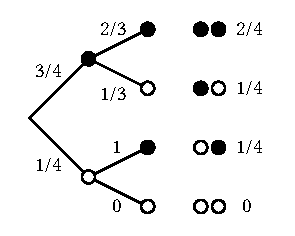
\includegraphics[width=50mm]{img/Baumdiagramm-Urne.pdf}
\caption{Baumdiagramm zur Ziehung aus der Urne}
\label{fig:Baumdiagramm-Urne}
\end{center}
\end{figure}

\noindent
Um die erste Pfadregel für Experimente mit mehr als zwei Stufen bestätigen
zu können, müssen wir zunächst ein paar Vorbetrachtungen machen.
Zunächst wird sich die Frage auftun, wie man bedingte Wahrscheinlichkeiten
von bedingten Wahrscheinlichkeiten bildet. Bei fester Bedingung $B$
bildet die bedingte Wahrscheinlichkeit wiederum ein Wahrscheinlichkeitsmaß,%
\[P_B\colon\Omega\to\R,\quad P_B(A) := P(A\mid B).\]
Diesbezüglich kann man nun von $P_B(A\mid C)$ reden. Allerdings findet
sich hierzu die Umformung%
\[P_B(A\mid C) = \frac{P_B(A\cap C)}{P_B(C)}
= \frac{\frac{P(A\cap B\cap C)}{P(B)}}{\frac{P(B\cap C)}{P(B)}}
= \frac{P(A\cap B\cap C)}{P(B\cap C)} = P(A\mid B\cap C).\]
Das heißt, die Schachtelung von bedingten Wahrscheinlichkeiten stimmt
mit der bedingten Wahrscheinlichkeit unter konjunktiver Verbindung der
Bedingungen, ausgedrückt als Schnittmenge, überein. Für $P(A\mid B\cap C)$
ist auch die Schreibweise $P(A\mid B,C)$ geläufig.

\subsection{Gesetz der totalen Wahrscheinlichkeit}

\begin{Satz}[Gesetz der totalen Wahrscheinlichkeit]%
\label{Gesetz-der-totalen-Wkt}\newlinefirst
Es sei $\setsystem Z$ eine Zerlegung der Ergebnismenge $\Omega$ in
paarweise disjunkte Mengen $B\in\setsystem Z$. Dann gilt
\[P(A) = \sum_{B\in\setsystem Z}P(A\mid B)P(B).\]
\end{Satz}
\begin{Beweis}
Es findet sich die Umformung
\begin{align*}
P(A) &= \textstyle P(A\cap\Omega) = P(A\cap\bigcup_{B\in\setsystem Z} B)
= P(\bigcup_{B\in\setsystem Z} (A\cap B))\\
&=\textstyle\sum_{B\in\setsystem Z} P(A\cap B)
= \sum_{B\in\setsystem Z} P(A\mid B)P(B).\,\qedsymbol
\end{align*}
\end{Beweis}

\newpage
\subsection{Satz von Bayes}

\begin{Satz}[Satz von Bayes]\label{Satz-von-Bayes}\newlinefirst
Es gilt $P(A\mid B) = \frac{P(A)}{P(B)}P(B\mid A)$, sofern $P(A)\ne 0$ und $P(B)\ne 0$.
\end{Satz}
\begin{Beweis}
Bestätigt sich mit der kurzen Rechnung
\[P(A\mid B) = \frac{P(A)}{P(A)}\frac{P(A\cap B)}{P(B)}
= \frac{P(A)}{P(B)}\frac{P(A\cap B)}{P(A)}
= \frac{P(A)}{P(B)}P(B\mid A)\,\qedsymbol\]
\end{Beweis}

\noindent
\strong{Anwendungsbeispiel: Beurteilung diagnostischer Tests.}
Zu einer bestimmten Krankheit wurde ein Testverfahren entwickelt.
Es weist eine \emph{Sensitivität} von 98\,\% auf. Das heißt, würde man
eine sehr große Zahl von ausschließlich tatsächlich erkrankten
Individuen testen, würde dieser Anteil als krank erkannt.
Weiterhin weist es eine \emph{Spezifität} von 97\,\% auf. Das heißt, würde
man eine sehr große Zahl von ausschließlich gesunden Individuen testen,
würde dieser Anteil als gesund erkannt. Aufgrund sowohl hoher Sensitivität
als auch hoher Spezifität darf man das Verfahren als recht zuverlässig
befinden.

Die Krankheit habe nun in der Bevölkerung eine Prävalenz von
1\,\%. Es wird ein zufälliges Individuum getestet. Das Ereignis $K$, dass
dieses Individuum krank ist, besitzt also die Wahrscheinlichkeit
$P(K)=0.01$. Es bezeichne $T^+$ bzw. $T^-$ das Ereignis, dass der Test
positiv bzw. negativ ausfällt. Es gilt $P(T^+\mid K)=0.98$ gemäß
der Sensitivität und $P(T^-\mid K^\compc)=0.97$ gemäß der Spezifität
des Tests.

Gesucht ist die Wahrscheinlichkeit $P(K\mid T^+)$, dass das Individuum
bei positivem Testergebnis in Wirklichkeit krank ist.

Im Zuge der disjunkten Zerlegung $\Omega = K\cup K^\compc$ gilt zunächst
\begin{align*}
P(T^+) &= P(T^+\mid K)P(K) + P(T^+\mid K^\compc)P(K^\compc)
\end{align*}
gemäß Satz \ref{Gesetz-der-totalen-Wkt}. Im Zuge der disjunkten
Zerlegung $\Omega = T^+\cup T^-$ gilt außerdem
\[P(\Omega\mid K^c) = P(T^+\mid K^\compc)+P(T^-\mid K^\compc)=1.\]
Via Satz \ref{Satz-von-Bayes} findet sich somit allgemein
\[P(K\mid T^+) = \frac{P(K)}{P(T^+)}P(T^+\mid K) =
\dfrac{1}{1+\dfrac{(1-P(T^-\mid K^\compc))(1-P(K))}{P(T^+\mid K)P(K)}}.\]
Wir berechnen speziell $P(K\mid T^+)\approx 0.25$. Obgleich der
Test recht genau erscheint, ist $P(K\mid T^+)$ aufgrund der
geringen Prävalenz recht niedrig.

Angenommen, bei der Krankheit handelt es sich um eine Infektionskrankheit.
In Bezug auf einen Hotspot, von dem man die lokale Prävalenz von
10\,\% in Erfahrung gebracht hat, ergibt sich immerhin $P(K\mid T^+)\approx 0.78$.
Das Testergebnis ist also nicht für sich allein aussagekräftig, sondern
wesentlich von der Prävalenz der Krankheit in der betrachteten Gruppe abhängig.

\subsection{Bayessche Inferenz}

Ich möchte im Fortgang noch eine dem subjektiven Wahrscheinlichkeitsbegriff
entstammende Sichtweise auf die Umstände einnehmen. Unter dieser berechnen
wir, wie sich die Wahrscheinlichkeit einer Hypothese bei Erhalt neuer
Information aktualisiert.

Wir haben eine \emph{Hypothese} $H$, von der wir nicht wissen, ob sie
stimmt. Allerdings ist bekannt, dass diese mit $P(H)$ eintritt, die man
die \emph{a-priori}"=Wahrscheinlichkeit nennt. Nun liegt eine neue
Information vor, die die \emph{Evidenz} $E$ schafft. Das heißt,
wir befinden uns in einer Situation, in der $E$ bereits beobachtet wurde,
was aber nur im Anteil $P(E)$ der Fälle passiert. Gefragt ist nun,
wie man $P(H)$ aktualisieren muss, um zu $P(H\mid E)$ zu gelangen,
die man die \emph{a-posteriori}"=Wahrscheinlichkeit nennt. Die
Aktualisierung vermittelt der Faktor $\frac{P(E\mid H)}{P(E)}$, so
dass sich der Satz von Bayes in der Form
\[P(H\mid E) = \frac{P(E\mid H)}{P(E)}P(H)\]
darstellt. Im zuvor diskutierten Beispiel zur Beurteilung diagnostischer
Tests war $H:=K$ die Hypothese und $E:=T^+$ die Evidenz.

In komplizierteren Situationen kann die Handhabung von Wahrscheinlichkeiten
bei bayesschen Rechnungen umständlich werden. Eine dienliche Alternative
besteht darin, mit \emph{Chancen} statt Wahrscheinlichkeiten zu arbeiten.

\begin{Definition}[Chance]\newlinefirst
Zu einer Wahrscheinlichkeit $P(A)\ne 1$ heißt $R(A):=\frac{P(A)}{1-P(A)}$,
also das \emph{Ratio} aus Wahrscheinlichkeit und Gegenwahrscheinlichkeit,
die \emph{Chance}, engl. \emph{odds}, des Ereignisses $A$.
\end{Definition}

\noindent
Insofern diese Gleichung zu $P(A)=\frac{R(A)}{1+R(A)}$ äquivalent umformbar
ist, gehört zu jeder Wahrscheinlichkeit genau eine Chance und umgekehrt.

Im näheren Blick auf die Regel von Bayes fällt auf, dass die
A"=priori"=Wahrscheinlichkeit in die Berechnung des Aktualisierungsfaktors
einfließt, was man als verwickelt empfinden mag. Wie man unschwer
nachrechnet, lässt sich die Regel von Bayes nun aber auch in der Form
\[R(H\mid E) = \frac{P(E\mid H)}{P(E\mid H^\compc)}R(H) = \frac{P(E\mid H)}{1-P(E^\compc\mid H^\compc)}R(H)\]
fassen, genannt die \emph{Chancen"=Form}, engl. \emph{odds form}.
In Bezug auf die diagnostischen Tests stellt sich dieser Sachverhalt dar als
\[R(H\mid E) = \frac{\text{Sensitivität}}{1-\text{Spezifität}}R(H).\]
Die A"=posteriori"=Chance $R(H\mid E)$ ergibt sich hier ebenfalls über
einen Aktualisierungsfaktor, genannt \emph{Bayes"=Faktor}, aus der
A"=priori"=Chance $R(H)$, der aber im Unterschied zur ursprünglichen
Fassung nicht mehr selbst abhängig von dieser ist. Als weiterer
Vorteil ergibt sich hierbei, dass sequentielles Aktualisieren in Bezug
auf eine Reihe Evidenzen durch simples Multiplizieren mit den jeweiligen
Bayes"=Faktoren vorgenommen werden darf. Hat man nämlich zwei
Evidenzen $E_1,E_2$ gesammelt, die sowohl unter $H$ als auch unter $H^\compc$
stochastisch unabhängig sind, also nichts miteinander zu tun haben,
ergibt sich unmittelbar die Umformung
\[R(H\mid E_2\cap E_1) = \frac{P(E_2\cap E_1\mid H)}{P(E_2\cap E_1\mid H^\compc)}R(H)
= \frac{P(E_2\mid H)}{P(E_2\mid H^\compc)}
\frac{P(E_1\mid H)}{P(E_1\mid H^\compc)}R(H).\]
Es ist aber Obacht geboten, $E_1,E_2$ nicht irrtümlich für sich allein
als stochastisch unabhängig zu befinden. Frequentistisch gesehen darf man
sich den Sachverhalt wie ein dreistufiges Zufallsexperiment vorstellen.
Zum Beispiel mit $H$ für \emph{ist krank} und $E_i$ für \emph{Test $i$ ist
positiv}. Im ersten Teilexperiment wird ein zufälliges Individuum aus der
Population ausgewählt, im zweiten der erste Test, im dritten der zweite
Test durchgeführt. Weiterhin sind $E_1,E_2$ allem Wissen nach unter $H$
unabhängig. Ohne Bedingung $H$ hat man es aber sowohl mit kranken
als auch gesunden Individuen zu tun. Betrachten wir dazu eine Population
von einer Mio. Individuen. Der erste Test siebt aus dieser eine gewisse
Zahl aus, die sich in $E_1$ versammeln. Diese Gruppe besitzt aber einen
höheren relativen Anteil an Kranken, so dass sich unter dieser die
Wahrscheinlichkeit für $E_2$ erhöht. Wir haben also $P(E_2\mid E_1) > P(E_2)$.
Wären $E_1,E_2$ unabhängig, müsste aber $P(E_2\mid E_1)=P(E_2)$ gelten.

Formal ist die zweite Pfadregel bzw. das Gesetz der totalen
Wahrscheinlichkeit anzuwenden, das macht
\[P(E_i) = P(E_i\mid H)P(H) + P(E_i\mid H^\compc)P(H^\compc).\]
Diese Gleichung verdeutlicht, wie $P(H)$ sowie $P(H^\compc)$ mit
in die Berechnung einfließen. Letztlich lässt sich damit ein konkretes
Beispiel rechnen, das als Gegenbeispiel die Unabhängigkeit von $E_1,E_2$
widerlegt.

\subsection{Bayessche Parameterschätzung}

Die bayessche Statistik ist ebenfalls zur Parameterschätzung dienlich.
Hierbei stellt man sich einen unbekannten Parameter vor, der aufgrund
von Unkenntnis anfangs zum Beispiel durch die Gleichverteilung
beschrieben wird. Das heißt, alle infrage kommenden Parameterwerte
seien gleich wahrscheinlich. Via neuer empirischer Evidenz wird nun
gemäß Bayes die Aktualisierung der Verteilung vorgenommen. Nun sollte
der wahre Parameter bei hinreichend starker Evidenz dort liegen, wo
sich die Verteilung konzentriert. Ich will den Sachverhalt anhand eines
vergleichsweise einfachen Beispiels näher erklären.

Es liege eine gut durchmischte Urne mit $s$ schwarzen und $w$ weißen
Kugeln vor. Aus der Urne wird eine zufällige Kugel gezogen. Es stehe
$X$ für das Ergebnis der Ziehung, mit $X=0$ für \emph{schwarz}, und
$X=1$ für \emph{weiß}. Insofern $s$ von insgesamt $s+w$ Kugeln für
$X=0$ günstig sind, bzw. $w$ für $X=1$, ergibt sich
\[P(X=0)=\frac{s}{s+w},\quad P(X=1)=\frac{w}{s+w}.\]
Alice teilt Bob die Anzahl $s$ der schwarzen Kugeln mit. Sie offenbart
ihm jedoch nicht die wahre Anzahl $w_0\in\{0,\ldots,N-1\}$ der
weißen. Nun darf Bob einmal aus der Urne ziehen, erhält damit die
Evidenz $X=x$, mit $x\in\{0,1\}$, bspw. konkret $X=0$. Wie verändert
sich dadurch Bobs Einschätzung, wie wahrscheinlich eine bestimmte Anzahl
$w$ von weißen Kugeln ist?

Bob nimmt die Anzahl der weißen Kugeln aus seiner Sicht als Zufallsgröße
$W$ an. Da bei Bob anfangs völlige Unkenntnis herrscht, nimmt
er die Gleichverteilung $P(W=w)=\frac{1}{N}$ als A"=priori"=Verteilung
an. Unter Voraussetzung $W=w$ weiß Bob die Wahrscheinlichkeit für
$X=0$, denn dann berechnet sich diese so, als wäre $w$ bekannt.
Das heißt, man hat $P(X=0\mid W=w)=\frac{s}{s+w}$. Hiermit bestimmt
Bob die aktualisierte Verteilung mit der Regel von Bayes zu
\[P(W=w\mid X=0) = \frac{P(X=0\mid W=w)}{P(X=0)}P(W=w).\]
Der Nenner des Aktualisierungsfaktors berechnet sich hierbei wieder mit
dem Gesetz der totalen Wahrscheinlichkeit als
\[P(X=0) = \sum_{k=0}^{N-1}P(X=0\mid W=k)P(W=k).\]
Die Kodierung der gezogenen Kugelfarbe als Zahl $x\in\{0,1\}$ gestattet
im Weiteren die geschickte Zusammenfassung
\[P(W=w\mid X=x) = \frac{(1-x)s+xw}{s+w}
= \Big(\frac{s}{s+w}\Big)^{1-x}\Big(\frac{w}{s+w}\Big)^x.\]
Sehr dienlich sein wird uns hierbei die letzte Form.

Nun ist die einzelne Ziehung nicht sonderlich Aufschluss gebend über die
wahre Anzahl. Daher sei es Bob im Weiteren gestattet, $n$ mal eine
Kugel mit zurücklegen zu ziehen, womit er den Stichprobenvektor
$x=(x_1,\ldots,x_n)$ erhält. Wir notieren zur Abkürzung
$E_i:=\{X_i=x_i\}$. Aufgrund der stochastischen Unabhängigkeit von
$E_1,E_2$ unter der Bedingung $W=w$ ergibt sich die Umformung
\begin{align*}
P(W=w\mid E_1\cap E_2) &= \frac{P(E_1\cap E_2\mid W=w)}{P(E_1\cap E_2)}P(W=w)\\
&= \frac{P(E_2\mid W=w)P(E_1\mid W=w)}{P(E_2\mid E_1)P(E_1)}P(W=w).
\end{align*}
Via $P(W=w\mid E_1) = \frac{P(E_1\mid W=w)}{P(E_1)}P(W=w)$
vereinfacht sich dies zu
\[P(W=w\mid E_1\cap E_2)
= \frac{P(E_2\mid W=w)}{P(E_2\mid E_1)}P(W=w\mid E_1).\]
Demnach darf das Aktualisieren der Wahrscheinlichkeit sequentiell
unternommen werden. Hierbei nimmt die im ersten Schritt ermittelte
A"=posteriori"=Verteilung im zweiten Schritt die Rolle der
A"=priori"=Verteilung ein.

Zur Berechnung ist auf den Nenner wieder das Gesetz der totalen
Wahrscheinlichkeit anzuwenden, das macht
\[P(E_2\mid E_1) = \sum_{k=0}^{N-1}P(E_2\mid E_1,W=k)P(W=k\mid E_1).\]
Letztlich gilt noch $P(E_2\mid E_1,W=k)=P(E_2\mid W=k)$ aufgrund der
Unabhängigkeit von $E_1,E_2$ unter $W=k$.

In ganz analoger Überlegung findet sich allgemeiner die Rekurrenz
\[P(W=w\mid A_i) = \frac{P(E_i\mid W=w)}{P(E_i\mid A_{i-1})}P(W=w\mid A_{i-1})\]
mit $A_0:=\Omega$ und $A_i := E_i\cap A_{i-1}$.

Indessen verhält es sich so, dass das Ziehen der Kugeln ein $n$"=stufiges
Bernoulli"=Experiment darstellt. Die Summe $Y:=\sum_{i=1}^n X_i$ ist
somit unter $W=w$ binomialverteilt, das heißt,
\[P(Y=y\mid W=w) = \binom{n}{y}p^y(1-p)^{n-y}\]
mit $p:=\frac{w}{s+w}$. Es tut sich jetzt die Frage auf, welcher der
beiden Ansätze, $X=x$ oder $Y=y$, besser schätzt. Die Antwort darauf
lautet \emph{keiner}. Beide führen exakt zur selben Verteilung.

Statt der sequentiellen Rechnung lässt sich die A"=posteriori"=Verteilung
nämlich auch in einem Rutsch berechnen. Dazu formen wir die
Likelihood um zu
\begin{gather*}
\textstyle P(X=x\mid W=w) = P(\bigcap_{i=1}^n E_i\mid W=w)
= \prod_{i=1}^n P(E_i\mid W=w)\\
= \textstyle\prod_{i=1}^n p^{x_i}(1-p)^{1-x_i}
= p^{\sum_{i=1}^n x_i}(1-p)^{\sum_{i=1}^n (1-x_i)}
= p^y (1-p)^{n-y}.
\end{gather*}
Demgemäß berechnet sich die Verteilung zu
\begin{align*}
P(W=w\mid X=x) &= \frac{P(X=x\mid W=w)}{P(X=x)}P(W=w)\\
&= \frac{p^y (1-p)^{n-y}}{\sum_{k=0}^{N-1} p_k^y (1-p_k)^{n-y}P(W=k)}P(W=w)
\end{align*}
mit $p:=\frac{w}{s+w}$ sowie $p_k:=\frac{k}{s+k}$. Es bestätigt sich nun
\[P(W=w\mid Y=y) = P(W=w\mid X=x),\]
da sich der Binomialkoeffizient herauskürzt.

Bislang blieb vage, welche ontologische Bedeutung der Zufallsgröße $W$
zukommt, zumal die wahre Anzahl weißer Kugeln eine feste, wenn auch
unbekannte Größe ist. Aus Bobs subjektivistischer Perspektive liegt
darin kein Widerspruch. Für ihn modelliert die A"=priori"=Verteilung die
anfängliche Unsicherheit über die wahre Anzahl. Die A"=posteriori"=Verteilung
stellt dahingehend seine verringerte Unsicherheit, sein aktualisiertes,
durch Evidenz informiertes Wissen dar.

Eine andere Deutung, die ohne subjektive Glaubensgrade auskommt,
ergibt sich durch einen Perspektivwechsel. Stellen wir uns Sofie -- Deus ex
Machina -- als übergeordnete Instanz vor, die das gesamte Szenario als zweistufiges
Zufallsexperiment entworfen hat. Im ersten Schritt wählt Sofie für Alice
eine zufällige Urne, indem sie die Anzahl der weißen Kugeln als
gleichverteilte Zufallszahl erzeugt. Im zweiten Schritt lässt sie Bob die
Stichprobe ziehen.

In diesem frequentistischen Rahmen ist $W$ eine »echte« Zufallsgröße.
Sofie sieht sich an ihrem Computer dazu befähigt, den gesamten Vorgang
beliebig oft  zu wiederholen, und die berechneten bedingten
Wahrscheinlichkeiten besitzen eine klare Häufigkeitsdeutung.

Als adäquate Ergebnismenge des Experiments haben wir
\[\Omega = \{0,\ldots, N-1\}\times\{0,1\}^n.\]
Die Zufallsgrößen deuten sich dahingehend als die Projektionen
\[\begin{array}{@{}c@{}l@{\quad}c@{}l@{}}
W&\colon\Omega\to\{0,\ldots,N-1\}, & W(w,x) &{}:= w,\\[3pt]
X&\colon\Omega\to\{0,1\}^n, & X(w,x) &{}:= x.
\end{array}\]
Alle Rechnungen bleiben hierbei natürlich unverändert gültig.

Sofie führt das Experiment eine Million mal durch. Mit einer
Häufigkeit $H_w$ wird eine Urne mit $w$ Kugeln gezogen, mit einer
Häufigkeit $H_y$ kommt die Summe $y=\sum_{i=1}^n x_i$ vor, und mit
einer Häufigkeit $H_{wy}$ tritt beides gleichzeitig ein. Sofern nicht
gerade $H_y=0$ ist, sollte gelten
\[\frac{H_{wy}}{H_y}\approx P(W=w\mid Y=y).\]
Zugleich konzentriert sich die Verteilung für eine große Stichprobenlänge
$n$ jeweils um die wahre Anzahl weißer Kugeln.

Eine bedeutsame Beobachtung ist hier, dass Bobs subjektive Sichtweise und
Sofies frequentistisches Experiment zu exakt derselben mathematischen
Berechnung führen. Die Debatte, welche Interpretation die »richtige« ist,
tritt in den Hintergrund. Stattdessen rückt der formale Modellcharakter
in den Vordergrund.

Wir haben es hier mit einem \emph{statistischen Modell} zu tun, dessen
Modellannahmen der Parameterraum, die A"=priori"=Verteilung und die
Likelihood"=Funktion sind. Im gegebenen Beispiel wirken sie durch die
Problemstellung natürlich, in der Praxis müssen sie jedoch sorgfältig
begründet werden.

Sofies übergeordnete Sicht stellt somit keine »objektive Wahrheit« dar,
sondern geht selbst mit den Modellannahmen einher -- sie ist eine
konstruierte Geschichte, die eine frequentistische Rechtfertigung für
den bayesschen Ansatz liefern soll.

Wir wollen diesbezüglich eine moderne Position einnehmen. Zur Ideenfindung
für den Modellansatz sei es uns gestattet, nach Belieben zwischen der
subjektivistischen und der frequentistischen Sichtweise hin und her
zu wechseln. Daraufhin behandeln wir das aufgestellte Modell aber als
formalen Gegenstand, der mit den Mitteln der axiomatisch fundierten
Wahrscheinlichkeitsrechnung auf seine Eigenschaften untersucht wird.
Später wählen wir dann denjenigen Ansatz aus dem Werkzeugkasten, von dem wir
annehmen, er liefere unter den gegebenen Umständen die beste Schätzung.

